% This is samplepaper.tex, a sample chapter demonstrating the
% LLNCS macro package for Springer Computer Science proceedings;
% Version 2.21 of 2022/01/12
%
\documentclass[runningheads]{llncs}
%
\usepackage[T1]{fontenc}
% T1 fonts will be used to generate the final print and online PDFs,
% so please use T1 fonts in your manuscript whenever possible.
% Other font encondings may result in incorrect characters.
%
\usepackage{graphicx}
\usepackage{tikz}
\usetikzlibrary{positioning, shapes.geometric}
\usepackage{adjustbox}
% Used for displaying a sample figure. If possible, figure files should
% be included in EPS format.
%
% If you use the hyperref package, please uncomment the following two lines
% to display URLs in blue roman font according to Springer's eBook style:
%\usepackage{color}
%\renewcommand\UrlFont{\color{blue}\rmfamily}
%\urlstyle{rm}
%


\hyphenation{OpenStack}

\sloppy

\begin{document}
%
\title{Challenges and Solutions of Developing and
	Implementing a Novel Desktop-as-a-Service}
%
\titlerunning{Challenges and Solutions of Developing and
	Implementing a Novel DaaS}
% If the paper title is too long for the running head, you can set
% an abbreviated paper title here
%
\author{Christian Baun \and
	Johannes Bouché}
\author{Christian Baun\orcidID{0009-0004-9955-3752} \and
	Johannes Bouché\orcidID{0009-0009-8003-4019}
}

\authorrunning{C. Baun, J. Bouché}
% First names are abbreviated in the running head.
% If there are more than two authors, 'et al.' is used.
%
\institute{Faculty of Computer Science and Engineering,\\
	Frankfurt University of Applied Sciences,\\
	Nibelungenplatz 1, 60318 Frankfurt am Main, Germany
	\email{[christianbaun|johannes.bouche]@fb2.fra-uas.de}}
\maketitle              % typeset the header of the contribution

\begin{abstract}
	Desktop-as-a-Service (DaaS) is a cloud service category
	with tremendous potential for improving the everyday work
	of running and using applications.
	However, existing DaaS solutions have several drawbacks,
	which have limited the popularity of this service category in the past.
	Our novel DaaS solution, DESIGN, overcomes existing solutions limitations
	and offers significant benefits.
	It can potentially revolutionize how we use applications,
	supporting non-modified Linux and Windows applications
	with just a browser on the client side.
	This paper describes some of the knowledge we gained
	during the development because of the challenges
	we faced and the solutions we found.

	\keywords{DaaS \and Compatibility \and Performance \and Stability \and Usability}
\end{abstract}

\section{Introduction}
This paper discusses challenges during the development
and implementation of a novel Desktop-as-a-Service (DaaS) solution
called DESIGN that enables the deployment
and usage of unmodified Linux and Windows applications
in the same way as web applications
and can run inside public resources
but can also be deployed in a private context.
Since all interaction with DESIGN and the hosted applications
is done via a user's web browser,
the users can use any client, no matter what hardware or host operating system
it is compromised of.
A browser is the only software component required to use the novel DaaS service.

Undoubtedly, developing a feature-rich DaaS system is a complex task, riddled with numerous obstacles and challenges. This paper meticulously categorizes these challenges into compatibility, performance, stability, and usability. It reveals these obstacles and presents the solutions we devised to overcome them, along with the valuable lessons we learned in the process.

Therefore, this document discusses in Section~\ref{sec:relatedworkAbschnitt}
the related work on DaaS solutions from an academic perspective,
whereas Section~\ref{sec:RecommendDaaSarchitecture}
describes the state-of-the-art DaaS architecture DESIGN we designed and implemented.
Section~\ref{sec:AnalysisPossibleComponents} presents the most relevant challenges we faced,
analyses our options for handling these,
and describes the solution we found.
Finally, Section~\ref{sec:Conclusions} discusses conclusions
and includes directions for future work.


\section{Related Work}\label{sec:relatedworkAbschnitt}


DaaS has been a well-known service category since the emergence of cloud computing.
Still, it got much less attention in research and literature.
The challenges and obstacles when developing DaaS solutions,
rather than infrastructure (IaaS) and platform services (PaaS),
have seldom been discussed in the literature.

Celesti et al.~\cite{celesti2016improving} implemented in 2016 a DaaS
using the IaaS solution OpenStack~\cite{sefraoui2012openstack}
and analyzed the characteristics and performance aspects of using noVNC,
which is a client for the protocol Virtual Network Computing (VNC)
that is implemented in the Hypertext Markup Language (HTML) and JavaScript,
the protocol SPICE (Simple Protocol for Independent Computing Environments),
and the remote desktop gateway Apache Guacamole as solutions
for providing access to the desktop via a browser.
One focus of the paper is the redirection
of the sound interface of the virtual desktop.
The paper's authors conclude that Guacamole,
in combination with the Remote Desktop Protocol (RDP), is the best solution.
The authors evaluated the lag time for remote audio playback
in an Internet scenario by measuring the time between the automated initiation
of the live streaming using the media player software VLC
and the arrival of the music data by analyzing network traffic
via the monitoring software Wireshark.
When using Guacamole combined with the protocol RDP,
the average lag was around 750\,ms.
When using Guacamole combined with the protocol VNC,
the average lag was around 1750\,ms.
The paper also includes a short evaluation of the lag for video frames
represented by background color changes of a Java application.
Again, Guacamole and RDP offered
the best video performance with an average lag of around 300\,ms.
The configuration of Guacamole and VNC caused an average lag of around 500\,ms.

Magana et al.~\cite{magana2019remote} compared in 2019
the most popular remote desktop protocols and software implementations.
The authors analyzed five protocols:
PCoIP used in the Amazon WorkSpaces, RDP, TeamViewer, VNC,
and Citrix Independent Computing Architecture (ICA).
In the paper, the network transfer rate and its relation to the quality
experienced by the DaaS user are evaluated
by assuming three scenarios:
using an office software suite, web browsing, and video streaming.
One emphasis of the paper is comparing the transfer rate
of the different protocols for three scenarios.
In the Office Software Suite scenario,
the transfer rate is measured and compared
when performing several tasks like opening
and editing a document (typing), loading an image, and saving a document.
The web browsing scenario covers requesting three different web pages,
and for the video streaming scenario,
the same YouTube video file was viewed at different resolutions.
The authors conclude that RDP requires fewer downstream
and upstream network resources for all three scenarios.
Generally can be said, that protocols RDP and VNC
are among the most popular frame-buffer protocols
which are utilized in countless open-source and proprietary projects
for different operating systems.
Depending on the various quality levels of the many existing implementations,
it is difficult to generalize about the performance of the protocols,
as individual implementations may have better
or worse performance characteristics than expected.

Several works in literature have analyzed
the latency of Cloud gaming services that have, in some aspects,
similar requirements to DaaS offerings.
According to Lampe et al.~\cite{lampe2014assessing},
the latency of locally executed games is compromised of the following components:
\begin{itemize}
	\item Input lag caused by the controller device (e.g., mouse or keyboard).
	\item CPU time for processing the user input and the program itself.
	\item GPU time of the graphics processor for rendering the next frame.
	\item Time required for delivering the frame into the frame buffer.
	\item LCD response time (time required to display the frame on the screen).
\end{itemize}


In cloud gaming scenarios the following components increase latency further:
\begin{itemize}
	\item Transfer time (upstream) for sending the user input to the service provider.
	\item Time required for capturing the frames and encoding it as a video stream.
	\item Transfer time (downstream) for sending the video stream to the client.
	\item Time required for decoding the video stream back into a frame.
\end{itemize}

For every deployment scenario or cloud service category possible,
users expect a latency value that is not annoying
when interacting with the service and its applications.
Choy et al.~\cite{ChoyWongSimonRosenberg2012},
Claypool et al.~\cite{claypool2010latency},
and Jarschel et al.~\cite{jarschel2011evaluation}
consider a maximum tolerable latency, based on subjective tests,
being around 100\,ms.
This relatively low value sets the demand for a fast network interaction
between client and service and limits their maximum distance.
As mentioned in Clincy et al.~\cite{clincy2013subjective},
The former cloud gaming service provider OnLive specified in the year 2010
that the distance between the service provider and the consumer
should not be greater than 1000 miles (approx. 1600\,km) because otherwise,
the round-trip communications delay time between will be too long for video games.
A more in-depth comparison of
commercially available cloud gaming services is given
by Di Domenico et al.~\cite{di2021network}
or by Carrascosa et al.~\cite{carrascosa2022cloud}.
Additionally, implied delays and round-trips can be further reduced
by using more sophisticated transmission protocols
directly interacting with GPU drivers,
such as Moonlight~\cite{darcy2022latency,hanimplementation}.

On first thought, the latency requirements of a modern computer game
are hardly the same as those of a desktop application.
However, just as with computer games,
the lagging operation of desktop programs
has a negative impact on the user experience,
and with video conferencing or other graphics-intensive applications,
the utilization of resources and latency requirements
are very similar to computer games.

\section{Architecture}\label{sec:RecommendDaaSarchitecture}
% 
Figure~\ref{figure_architecture} shows the architecture
of our novel DaaS solution DESIGN
that can run unmodified Linux and Windows applications in Linux containers
(Native Linux applications and Native Windows applications compatible with Wine)
and virtual machines (Native Windows applications incompatible with Wine).
\begin{figure}
	\centering
	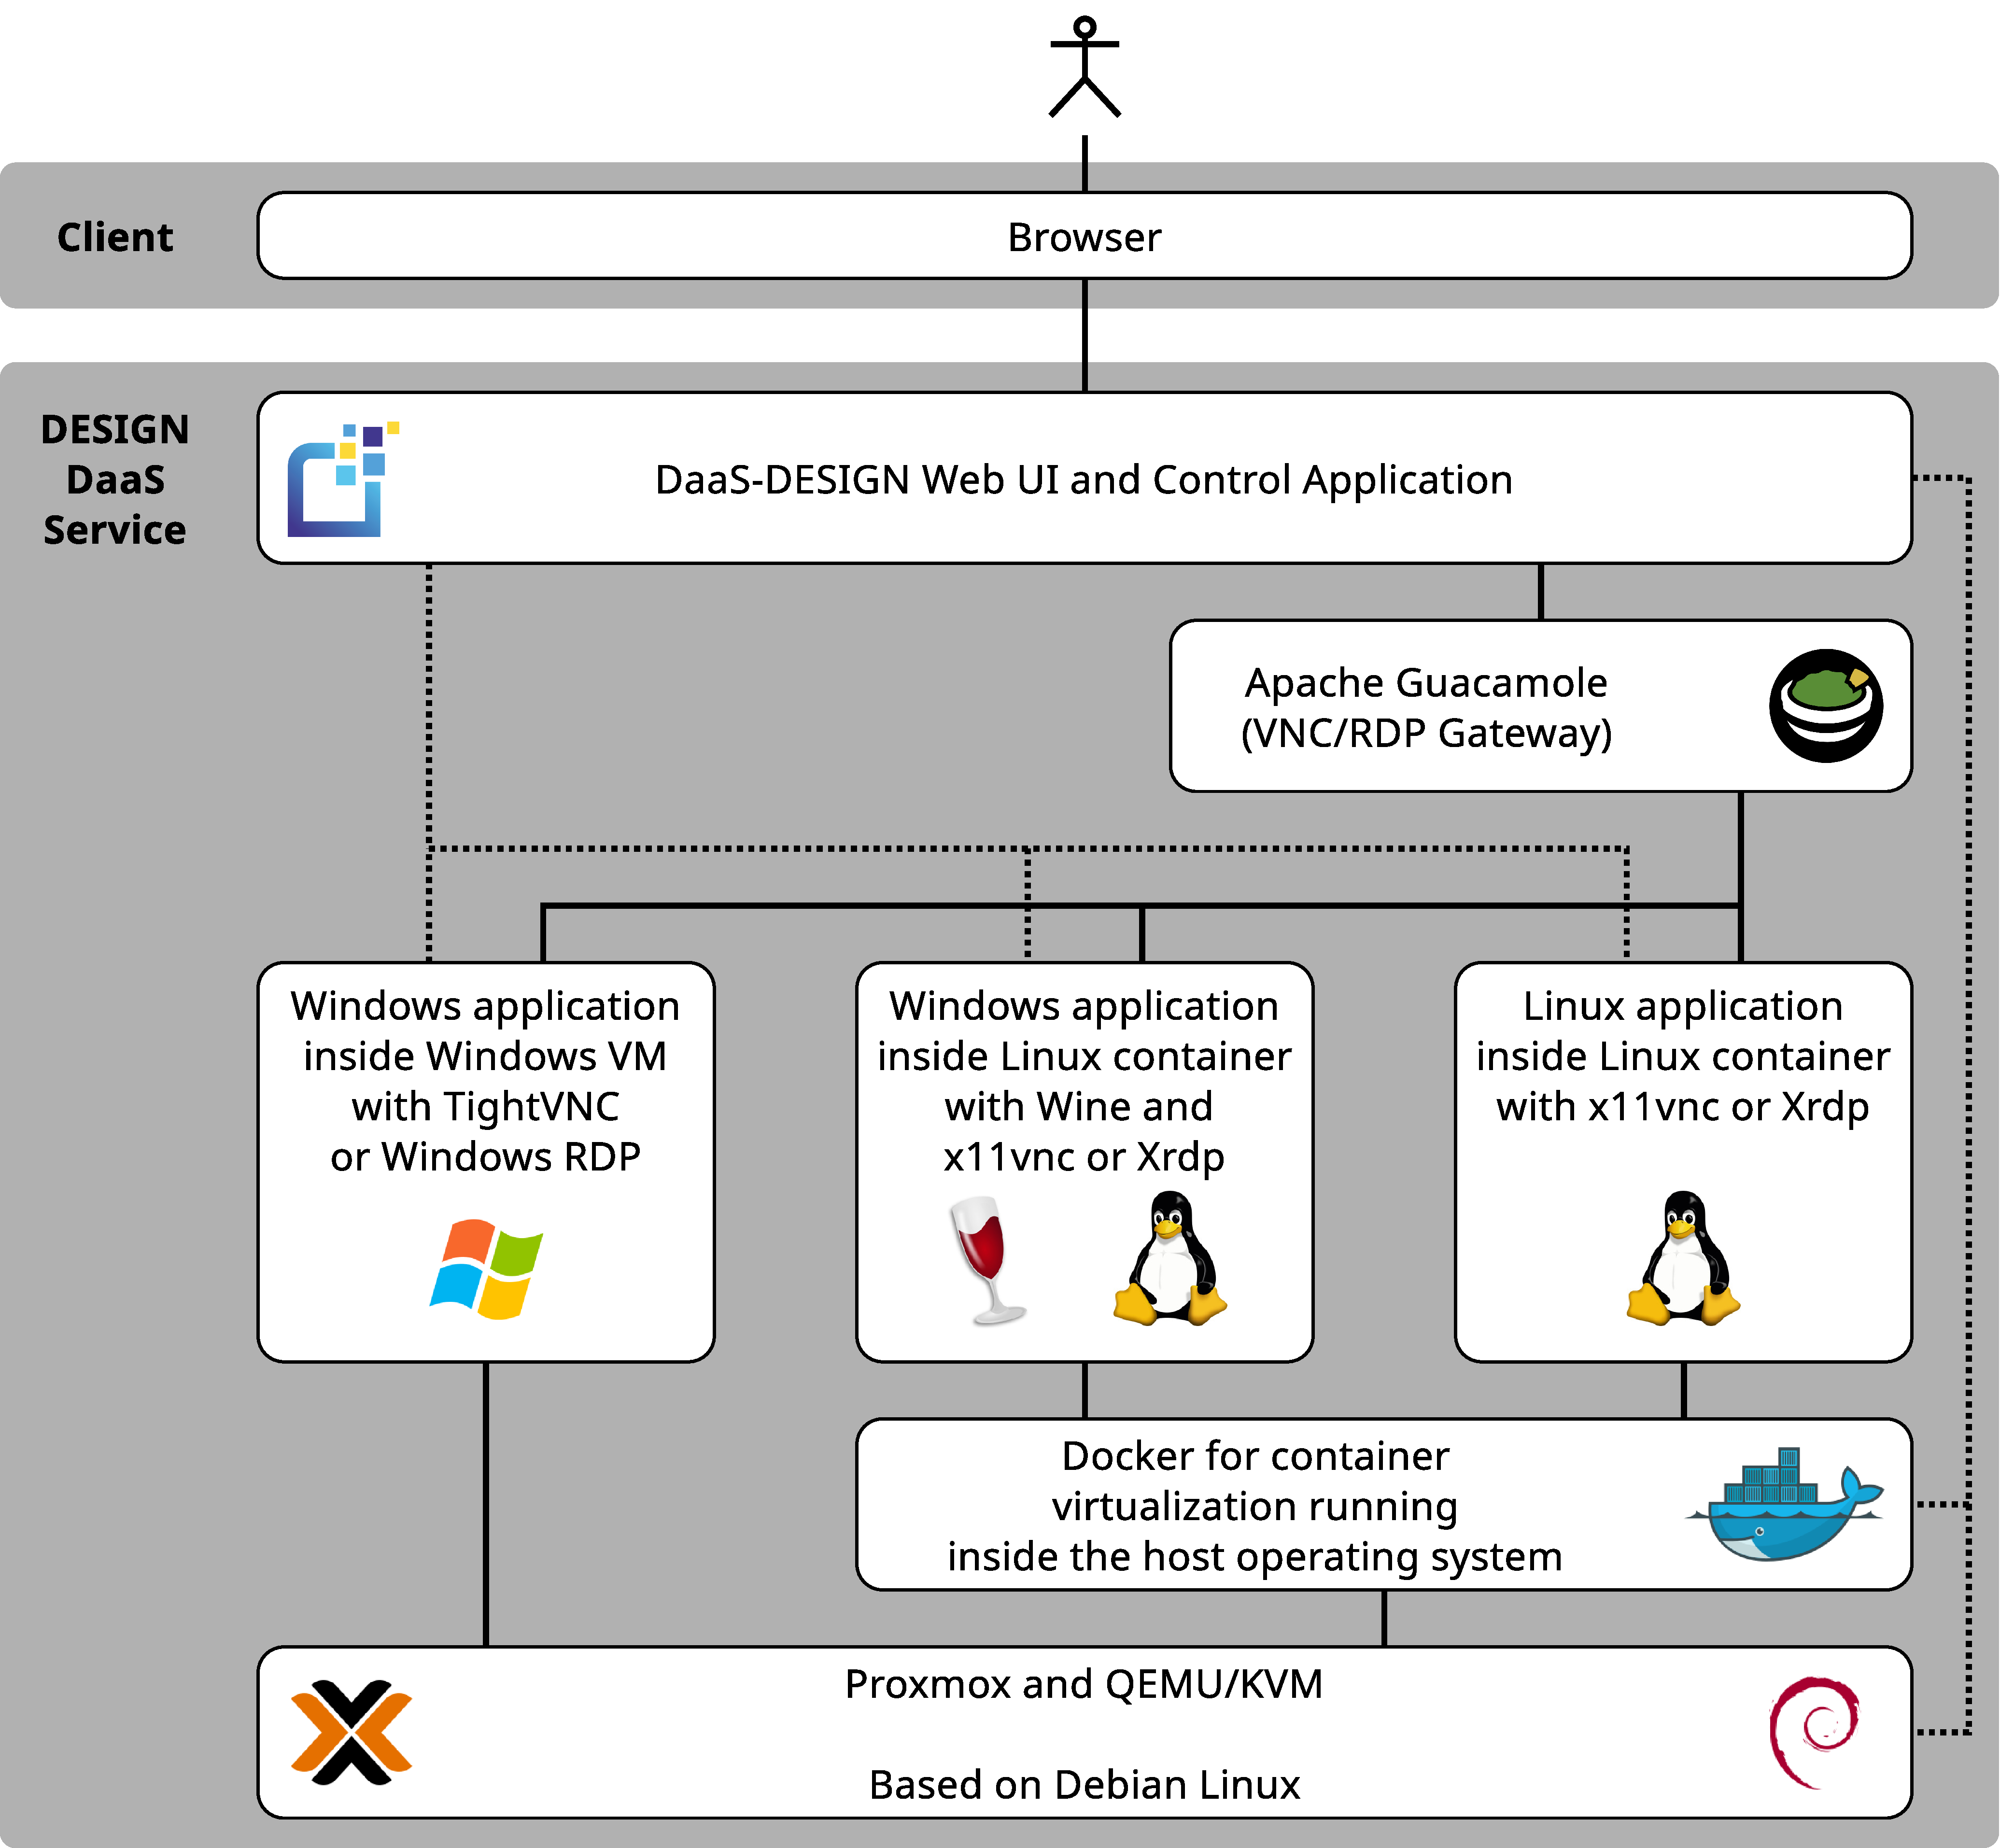
\includegraphics[width=.75\linewidth]{images/DaaS_DESIGN_Architecture_v12_english.pdf}
	\caption{Architecture of the novel DaaS DESIGN~\cite{OJCC_2023v8i1n01_Baun}.}
	\label{figure_architecture}
\end{figure}

The open-source server virtualization platform Proxmox VE runs bare-metal and offers virtual machines with the Kernel-based Virtual Machine (KVM) and container-based virtualization via LXC Linux container. Since the LXC API is, in comparison to the Docker API, rather poorly documented and lacks several features, we considered Docker a better container virtualization solution. A deployment of docker directly in the host-operating system or inside a virtual machine is both possible.

Exporting the graphical user interface of Linux and Windows applications
is possible using VNC or RDP protocols.
Free server implementations exist for both operating system families.
Since our DaaS solution focuses on exporting only the application's graphical user interface
and not full desktops -- a feature not all server implementations include --
the number of available projects and solutions is limited.
For Linux containers, the free software projects
x11vnc and Xrdp can be used in the DESIGN DaaS.
For Windows VMs, the free software TightVNC
and the Windows-internal RDP server can be used.

One of the main goals of DESIGN is to allow all interactions to be carried out
solely using a browser.
Thus, a broker or proxy software that mediates between the VNC or RDP
implementation and the browser is required.
The most advanced solution available
is the free software project Apache Guacamole, which supports VNC and RDP
and includes further relevant features regarding sound and printer support.

The core components of DESIGN are our self-developed Web UI
and the Control Application,
which carry out the communication between all service components.

Starting a virtual machine or container instance automatically includes an SSH service.
Our self-developed instance component waits
until the SSH service is ready to satisfy requests.
If applications are to be started or modifications are to be carried out,
the instance component sends these requests to the virtual machine or container.
Modification requests include resolution changes
and fetching host status information.

The self-developed instance component generally allows users
to carry out essential administration
and usage tasks that the operating system does not offer via a generalized API.

\section{Challenges and Solutions}\label{sec:AnalysisPossibleComponents}

While developing the novel DaaS platform DESIGN,
we faced multiple obstacles and challenges.
Each issue belongs to one of four categories:
compatibility, performance, stability, and usability.
This section presents the issues we faced,
the possible approaches we analyzed, and the solutions we chose.

\subsection{Compatibility}

The first relevant characteristic of a DaaS
that a user is confronted with
is the list of compatible applications.
In the best case,
all applications of all popular operating systems
can be integrated and used with such a novel platform.
Several DaaS projects and solutions from the last two decades
and similar concepts like web desktops
or webtops lacked native support for popular applications.

Examples worth mentioning in this context include eyeOS and SilveOS.
The project eyeOS~\cite{liu2012research,vidyabanu2011implementation}
simulates a desktop environment using HTML,
the scripting language PHP, JavaScript,
and the MySQL database management system.
The project SilveOS~\cite{garmpis2016design}
mimics the look and feel of a Windows desktop in the browser
using the discontinued application framework Microsoft Silverlight.
Despite being free software,
both solutions have never become widely
used since it is impossible to import
and use native Windows or Linux applications there.
All required applications have to be developed as web applications.
This limitation caused most potential users to lose interest in web desktops
because many popular native applications can hardly be replaced or re-developed,
and many feature-rich and well-established Software-as-a-Service (SaaS)
offerings like Microsoft Office 365 and Google Docs already exist.

A new DaaS is only accepted by a broad user group if it
enables the integration of native applications in an unchanged manner.
It is also desirable that a DaaS supports Linux and Windows applications
both to allow flexible working and make the operation
of a virtualization solution on the desktops unnecessary.
Ideally, it should also be possible to run native Mac OS applications.
However, this goal is difficult to achieve under legal conditions
due to the Mac OS operating system's licensing restrictions.

Further essential features for most users are printing, sound,
and compatibility with external storage media.

Guacamole supports redirecting audio, printing,
and disk access via the protocol RDP.
The printing feature does not allow access to local or remote printers;
instead, it allows users to print directly to PDF files,
which are received by the user's web browser.
As a prerequisite, the GhostScript interpreter
must be deployed on the Guacamole server.
File transfer over RDP supports Guacamole
by emulating a virtual disk drive that persistently stores data
on the Guacamole server.\footnote{\url{https://guacamole.apache.org/doc/1.5.5/gug/configuring-guacamole.html}}

Compared to RDP, the protocol VNC offers fewer features in Guacamole
since it does not support sound on its own.
However, Guacamole supports sound using
PulseAudio\footnote{On Linux operating systems,
	sound and microphone devices are accessed via sound servers like PulseAudio and PipeWire,
	which interact with the sound interface present in the kernel,
	e.g., Advanced Linux Sound Architecture (ALSA) or Open Sound System (OSS)}
as a workaround solution.
VNC also does not offer file transfer and access to external storage media.
Still, as a workaround solution, Guacamole supports file transfer
via the SSH File Transfer Protocol (SFTP),
which is an extension of the Secure Shell protocol (SSH).

\subsection{Performance}
Performance, from our viewpoint, stands out as the most crucial system property,
implying the influence of other  relevant properties,
such as user experience, system responsiveness, and overall efficiency.
Consequently, we encountered multifaceted challenges
that potentially intersected across several layers within our architecture
and which will be described in the following subsections.

\subsubsection{Infrastructure and Platform}
In general, it can be said that the chosen infrastructure, platform,
and utilized software combined may have the most impact on the overall resource consumption
and are therefore of major importance.
As a DaaS system combines all aspects of IaaS-, PaaS, and SaaS-based computation, each performance characteristic must be considered.

Regarding Infrastructure-as-a-Service (IaaS),
our solution generally offers the flexibility
to use either virtual machines or containers.
Scientific publications discussing relevant performance aspects of such systems
highlight the apparent advantage of a lightweight container solution
over virtual machines when identical programs are tested in both
environments~\cite{felter2015updated,potdar2020performance}.

This suggests that a container-based approach is likely preferable
if the choice is available.
However, not every application can be run
in a container-based environment,
so we maximize coverage of potential usecases
by offering both container-based and virtual machine-based application hosting.

Regarding Platform-as-a-Service (PaaS),
studies show that there is no dramatic difference in performance
when derivatives of operating systems are compared to each
other~\cite{balen2020performance,boras2020performance}.
Nevertheless, some derivatives are more lightweight and performant.
In contrast, comparing operating systems of different types
reveals more obvious results, particularly when considering
low-level operating system functionality implementations
such as interrupt handling, memory allocation, and boot
time~\cite{sulaiman2021comparison}.
Additional performance potentials can be leveraged
in cases where a Windows virtual machine can be replaced
with a container-based solution integrating 
wine~\cite{huang2012performance}.

For SaaS, performance largely depends on the underlying usage model
and the actual software being virtualized.
Depending on the use case, influential properties
such as multi-tenancy, provision strategies, or the virtualized data type
might be utilized to varying degrees, resulting in overall
better or worse performing systems~\cite{zhong2010virtualization}.

Despite the potential for usecase-specific optimization,
we emphasize that for DaaS systems,
coverage of a broad range of potential use cases is generally more favorable
than solving a particular use case most efficiently.
Therefore, we consider all user-facing desktop applications
as plausible candidates for migration to our systems,
rather than more complex distributed systems
for which tailored environments might be more suitable.


Figure~\ref{hosting_scenarios} visualizes the available hosting strategies for our platform.
We aim to support any Windows or Linux-based application in virtual machines
and any Linux- and Wine-based applications in container environments.

\begin{figure}
	\centering
	\begin{adjustbox}{width=\textwidth}
		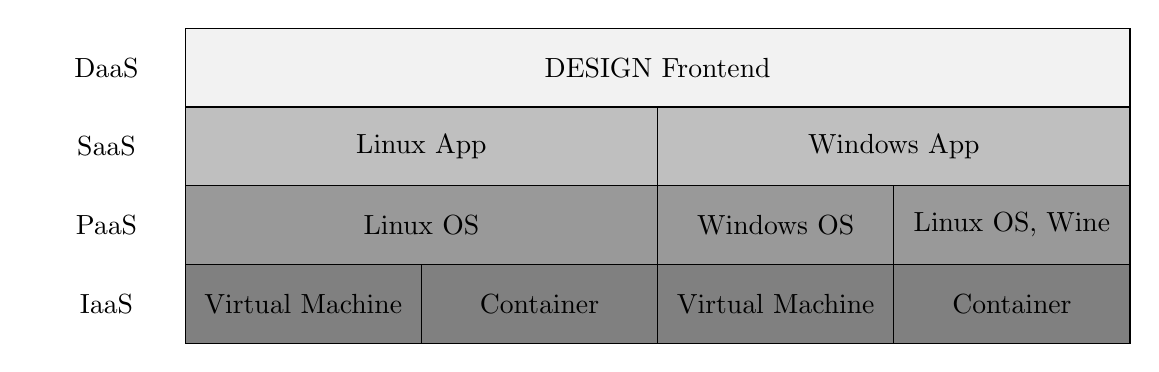
\begin{tikzpicture}[every node/.style={minimum height=1cm, align=center}]
			%Type Column
			\node[minimum width=2cm] at (-4,-2) {IaaS};
			\node[minimum width=2cm] at (-4,-1) {PaaS};
			\node[minimum width=2cm] at (-4,0) {SaaS};
			\node[minimum width=2cm] at (-4,1) {DaaS};
			% DaaS
			\node[draw, minimum width=12cm, fill=gray!10] at (3,1) {DESIGN Frontend};
			%Linux
			\node[draw, minimum width=6cm, fill=gray!50] at (0,0) {Linux App};
			\node[draw, minimum width=6cm, fill=gray!80] at (0,-1) {Linux OS};
			\node[draw, minimum width=3cm, fill=gray!100] at (-1.5,-2) {Virtual Machine};
			\node[draw, minimum width=3cm, fill=gray!100] at (1.5,-2) {Container};
			%Windows
			\node[draw, minimum width=6cm, fill=gray!50] at (6,0) {Windows App};
			\node[draw, minimum width=3cm, fill=gray!80] at (4.5,-1) {Windows OS};
			\node[draw, minimum width=3cm, fill=gray!80] at (7.5,-1) {Linux OS, Wine};
			\node[draw, minimum width=3cm, fill=gray!100] at (4.5,-2) {Virtual Machine};
			\node[draw, minimum width=3cm, fill=gray!100] at (7.5,-2) {Container};
		\end{tikzpicture}
	\end{adjustbox}
	\caption{Application hosting strategies.}\label{hosting_scenarios}
\end{figure}

\subsubsection{Network Latency and Bandwidth}
Network Latency and Bandwidth are crucial factors
in delivering web-based access to DaaS apps,
directly impacting system responsiveness experienced by users.
Supporting standardized frame-buffer protocols enables user interaction initially
and provide additional access to external devices like printers or USB sticks.
In cases involving, for example, video content transmission,
network bandwidth often becomes the main bottleneck,
especially with high-resolution video streams.
In contrast to that, when transmitting audio, mouse movements,
or keyboard inputs, network latency becomes more important.

Application-specific requirements can be managed to some extent
through protocol-inherent tuning parameters and compression algorithms.
Our solution, therefore, offers a range of tuning options
to adapt to different use cases on a per-user basis.

We utilize the Guacamole desktop gateway implementation,
supporting widely used frame-buffer protocols like VNC and RDP,
along with relevant tuning options.
Guacamole also enables audio support and integration with external devices
through a JavaScript-based web client (guacamole.js).
As depicted in figure~\ref{websocket_proxy},
the proxy component receives HTTP requests from guacamole.js
and is forwarded by the backend through WebSocket opcodes (Guacamole protocol).
These opcodes are then transmitted to the Guacamole daemon (guacd)
which in turn communicates to each instance
by using regular frame-buffer protocols (VNC or RDP).

However, integrating Guacamole into the system
requires consideration of additional factors besides the frame-buffer protocols itself.
Authentication mechanisms, for example, are essential in a DaaS context,
as users expect seamless authentication across the whole system
without multiple logins.
Additionally, safeguarding sensitive information like user passwords is crucial
for maintaining system security and user trust.
To mitigate the risk of unintended system manipulation, Guacamole was integrated
using a proxied approach and WebSockets.
This ensures that the credentials of a generated instance remain secret to the host system
while still providing authorized, passwordless access to the hosted application.

Moreover, the proxy mechanism enables support for other additional features
such as dynamic desktop resizing.
While Guacamole offers support for that by default in RDP, support for the VNC protocol is completely missing.
Nevertheless, the proxied approach enables intercepting all exchanged WebSocket opcodes
and by listening for size requests
the requested feature could be added
by directly interacting with the instance on another layer.

While these changes to the default Guacamole use case are necessary to align
with the underlying DaaS design requirements,
they also negatively impact overall system performance and responsiveness.
The integration as a proxy introduces additional network hops,
leading to noticeable delays in network communication.
Additionally, the protocol-level evaluation of opcodes further increases this delay,
potentially affecting perceived responsiveness
if resize requests take longer than expected.
However, despite the introduced overhead,
the solution still enables platform-independent
and seamless access for all defined DaaS use cases.

\begin{figure}
	\centering
	\begin{adjustbox}{width=\textwidth}
		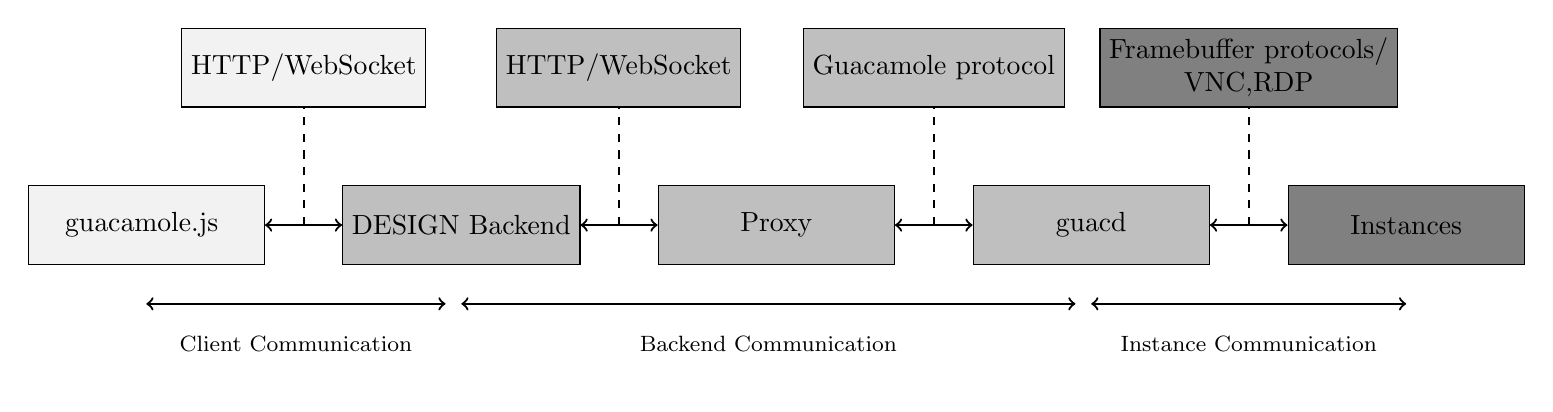
\begin{tikzpicture}[every node/.style={minimum height=1cm, align=center}]

			% Nodes center row
			\node[draw, minimum width=3cm, fill=gray!10] (browser) at (0,0) {guacamole.js };
			\node[draw, minimum width=3cm, fill=gray!50] (back) at (4,0) {DESIGN Backend};
			\node[draw, minimum width=3cm, fill=gray!50] (proxy) at (8,0) {Proxy};
			\node[draw, minimum width=3cm, fill=gray!50] (guacd) at (12,0) {guacd};
			\node[draw, minimum width=3cm, fill=gray!100] (inst) at (16,0) {Instances};
			% Arrows center row
			\draw[<->, thick, black] (browser.east) -- (back.west);
			\draw[<->, thick, black] (back.east) -- (proxy.west);
			\draw[<->, thick, black] (proxy.east) -- (guacd.west);
			\draw[<->, thick, black] (guacd.east) -- (inst.west);
			% Upper row
			\node[draw, minimum width=3cm, fill=gray!10] (client-backend) at (2,2) {HTTP/WebSocket};
			\node[draw, minimum width=3cm, fill=gray!50] (backend-proxy) at (6,2) {HTTP/WebSocket};
			\node[draw, minimum width=3cm, fill=gray!50] (proxy-guacd) at (10,2) {Guacamole protocol};
			\node[draw, minimum width=3cm, fill=gray!100] (guacd-inst) at (14,2) {Framebuffer protocols/\\VNC,RDP};
			% Dashed lines upper row
			\draw[-, dashed, thick, black] (2,0) -- (2,1.5);
			\draw[-, dashed, thick, black] (6,0) -- (6,1.5);
			\draw[-, dashed, thick, black] (10,0) -- (10,1.5);
			\draw[-, dashed, thick, black] (14,0) -- (14,1.5);
			% Arrow bottom row
			\draw[<->, thick, black] (0,-1) -- (3.8,-1) node[midway, below, font=\footnotesize] {Client Communication};
			\draw[<->, thick, black] (4,-1) -- (11.8,-1)node[midway, below, font=\footnotesize] {Backend Communication};
			\draw[<->, thick, black] (12,-1) -- (16,-1)node[midway, below, font=\footnotesize] {Instance Communication};
		\end{tikzpicture}
	\end{adjustbox}
	\caption{WebSocket Proxy Components.}\label{websocket_proxy}
\end{figure}

\subsubsection{Internal Processing and Communication}
Another critical aspect directly related to performance and responsiveness
is how data is internally processed, stored, and communicated.
This includes metadata collected and processed
and involves data exchange with all relevant backend services or instances.

Ensuring a satisfying user experience in a DaaS system
implies specific components to be available.
This includes access to all infrastructural backend services,
a databases, authentication services, filesystems, and network devices.
Additionally, a web server is integrated to provide relevant API endpoints
for frontend communication and WebSocket endpoints for the viewer.

Generally spoken, all of these components can potentially become bottlenecks
when handling high throughputs or large amounts of concurrent applications
and is especially true if all components are served from the same hardware.
Architecturally, all relevant components
must therefore be designed for distribution across different hosts.
However, keeping specific components directly on the host system
may still be required to ensure low-latency access.

From our observations, components requiring real-time and low-latency performance,
should physically be kept as close to the core hosting system as possible
as shown in figure~\ref{perf_internal_communication}.
This includes all data and communication relevant to
audio, video, mouse, and keyboard transmission,
as well as all backend services for hosting containers and virtual machines.
Ideally, these components should be hosted natively on the host system
for virtual network and hardware access
or at least be connected to the same physical network
to minimize network latencies.
All other components might be distributed to dedicated systems
if large user amounts and specific use cases have to be handled
but keeping them in close physical proximity
to the host remains prudent in smaller scales.

Although we can not yet provide a full-fledged performance analysis,
we already measured promising results in our local test environment.
Depending on the exact setup,
the solution provides
reasonable round-trip times and delays for each communication direction
visualized in figure~\ref{perf_internal_communication}.
In a minimal setup, we measured delays of around 10ms for client communication,
around 100ms for internal backend communication
but up to 1000ms for instance communication.
However, these numbers are only rough estimates
as certain optimization concepts remain to be implemented.
% Explanation delays: Half-way of a Roundtrip.
% We state 1000ms for instance-communication (500ms per connection, we make two, so 1000ms)
% We state 100ms for internal comm, which is a roundtrip of 200ms for auth divided by two, so 100ms
% 10ms for client delay we can take a clientside timestamp when sending request and a server side timestamp when the request is intially received.
% So we directly measure a deley, no rtt. The delay varias between 9 and 14ms, so we state roughly 10ms.
% In my newest tests this number goes up to 50ms, but thats ok for what we receive in advance.

\begin{figure}
	\centering
	\begin{adjustbox}{width=\textwidth}
		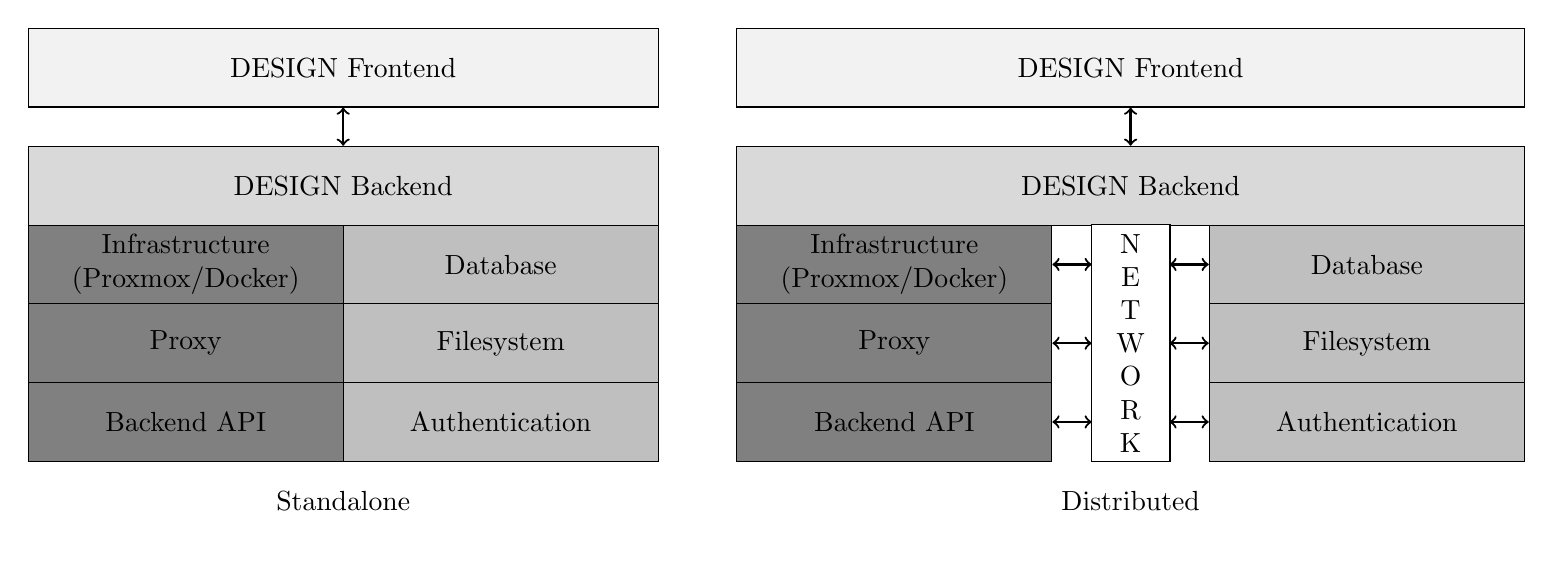
\begin{tikzpicture}[every node/.style={minimum height=1cm, align=center}]
			% Standalone Realtime
			\node[draw, minimum width=8cm, fill=gray!10] (singlefront) at (0,-0.5) {DESIGN Frontend};
			\node[draw, minimum width=8cm, fill=gray!30] (singleback) at (+0,-2) {DESIGN Backend};
			\node[draw, minimum width=4cm, fill=gray!100] at (-2,-3) {Infrastructure\\(Proxmox/Docker) };
			\node[draw, minimum width=4cm, fill=gray!100] at (-2,-4) {Proxy};
			\node[draw, minimum width=4cm, fill=gray!100] at (-2,-5) {Backend API};
			% Standalone Services
			\node[draw, minimum width=4cm, fill=gray!50] at (+2,-3) {Database};
			\node[draw, minimum width=4cm, fill=gray!50] at (+2,-4) {Filesystem};
			\node[draw, minimum width=4cm, fill=gray!50] at (+2,-5) {Authentication};
			%Standalone Caption
			\node[minimum width=8cm] (browser) at (0,-6) {Standalone};
			% Distributed Realtime
			\node[draw, minimum width=10cm, fill=gray!10] (distfront) at (10,-0.5) {DESIGN Frontend};
			\node[draw, minimum width=10cm, fill=gray!30] (distback) at (10,-2) {DESIGN Backend};
			\node[draw, minimum width=4cm, fill=gray!100] (inf) at (7,-3) {Infrastructure\\(Proxmox/Docker) };
			\node[draw, minimum width=4cm, fill=gray!100] (proxy) at (7,-4) {Proxy};
			\node[draw, minimum width=4cm, fill=gray!100] (api) at (7,-5) {Backend API};
			% Distributed Services
			\node[draw, minimum width=4cm, fill=gray!50] (db) at (13,-3) {Database};
			\node[draw, minimum width=4cm, fill=gray!50] (fs) at (13,-4) {Filesystem};
			\node[draw, minimum width=4cm, fill=gray!50] (auth) at (13,-5) {Authentication};
			% Network
			\node[draw, minimum width=1cm, minimum height=3cm, fill=white] (browser) at (10,-4) {N\\E\\T\\W\\O\\R\\K};
			% Distributed Caption
			\node[minimum width=10cm] (browser) at (10,-6) {Distributed};
			% Arrows back<->front
			\draw[<->, thick, black] (singleback.north) -- (singlefront.south);
			\draw[<->, thick, black] (distback.north) -- (distfront.south);
			% Arrows realtime
			\draw[<->, thick, black] (inf.east) -- ++(0.5,0);
			\draw[<->, thick, black] (proxy.east) -- ++(0.5,0);
			\draw[<->, thick, black] (api.east) -- ++(0.5,0);
			% Arrows services
			\draw[<->, thick, black] (db.west) ++(-0.5,0) -- ++(0.5,0);
			\draw[<->, thick, black] (fs.west) ++(-0.5,0) -- ++(0.5,0);
			\draw[<->, thick, black] (auth.west) ++(-0.5,0) -- ++(0.5,0);
		\end{tikzpicture}
	\end{adjustbox}
	\caption{Internal Communication Flow}\label{perf_internal_communication}
\end{figure}

\subsection{Stability}
Stability in DaaS applications is essential
for meeting the demands of continuous and time-critical operations
across diverse user scenarios.
Ensuring the stability of all system components during runtime is paramount
to maintain service continuity, handle growing user loads,
and transparent failure recovery while providing a seamless end-user experience.
These considerations are integral to our architectural concept,
directly impacting the operational integrity of the system
and its suitability for enterprise-level deployment and trust.

Therefore, key strategies, such as component redundancy, node scalability
as well as the internal communication concept
will be described in the following subsections.

\subsubsection{Scalability of Components}
Scalability in DaaS environments
can be approached through two fundamental methods: horizontal and vertical scaling.
Horizontal scaling (scale out), involves adding more machines or instances
to manage increased loads.
In contrast, vertical scaling (scale up),
adds more power (CPU, RAM) to existing 
machines~\cite{vaquero2011dynamically}.
While horizontal scaling offers flexibility
and is often preferred in cloud environments,
vertical scaling remains important for applications
requiring strong single-thread performance or low latencies.

To comply with both approaches,
we designed the system and its backend services
to be split into logical units that can be distributed across dedicated systems.
Each backend service receives a dedicated configuration
and can be accessed via hostname and port tuples.
By default, all backend services reside on the same host.
In a distributed context, services can be distributed to dedicated remote systems
to adhere to horizontal scaling principles.

Vertical scaling of DaaS nodes is not currently planned,
but administrators are free to use custom third-party toolchains,
such as GPU virtualization for vertical scaling on a per-host basis.
Although vertical scaling within a host
is beyond the scope of our research project,
scaling the instances hosted within the system is feasible for both dimensions.
For vertical scaling of instances, we provide appropriate parameters
and API endpoints to manipulate resource assignments,
allowing for arbitrary configurations.

For horizontal scaling of instances, the built-in mechanisms
of each backend service are automatically configured
and utilized to distribute instances across a pool of connected nodes.
Proxmox implements such mechanisms
for virtual machines as part of its `Proxmox VE High Availability (HA)' cluster.
Similar concepts can be integrated for containers with any backend service,
such as Kubernetes.
Within these clusters,
DaaS instances are entirely agnostic to their hosting system
and only need to be reachable
via a known hostname or IP as a single requirement.
As shown in figure~\ref{scale_objects_horizontal},
we provide a globally maintained state of data, authentication, and storage
which is accessible either by horizontally scaled backends and frontends
or otherwise,
by horizontally and vertically scaled instances in our DaaS object domain.

\begin{figure}
	\centering
	\begin{adjustbox}{width=\textwidth}
		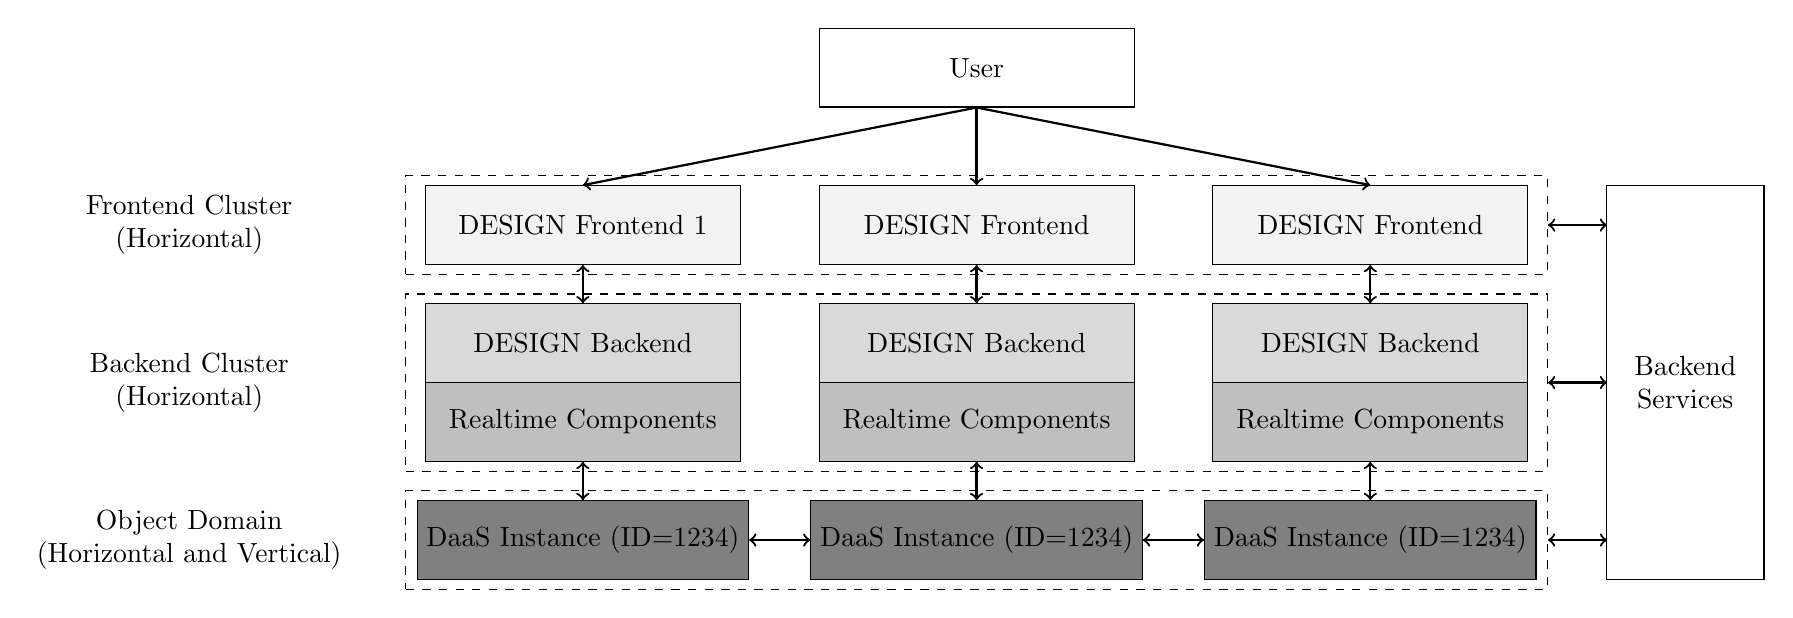
\begin{tikzpicture}[every node/.style={minimum width=4cm, minimum height=1cm, align=center}]

			% User
			\node[draw, minimum width=4cm] (user) at (5,1.5) {User};
			% Clusters
			\node[] at (-5,-0.5) {Frontend Cluster\\(Horizontal)};
			\node[] at (-5,-2.5) {Backend Cluster\\(Horizontal)};
			\node[] at (-5,-4.5) {Object Domain\\(Horizontal and Vertical)};

			% Node1
			\node[draw, fill=gray!10]  (front1) at (0,-0.5) {DESIGN Frontend 1};
			\node[draw, fill=gray!30]  (back1)  at (0,-2.0) {DESIGN Backend};
			\node[draw, fill=gray!50]  (real1)   at (0,-3.0) {Realtime Components};
			\node[draw, fill=gray!100] (inst1)  at (0,-4.5) {DaaS Instance (ID=1234)};
			% Node2
			\node[draw, fill=gray!10]  (front2) at (5,-0.5) {DESIGN Frontend};
			\node[draw, fill=gray!30]  (back2) at (5,-2.0) {DESIGN Backend};
			\node[draw, fill=gray!50]  (real2) at (5,-3.0) {Realtime Components};
			\node[draw, fill=gray!100] (inst2)  at (5,-4.5) {DaaS Instance (ID=1234)};
			% Node3
			\node[draw, fill=gray!10]  (front3) at (10,-0.5) {DESIGN Frontend};
			\node[draw, fill=gray!30]  (back3) at (10,-2.0) {DESIGN Backend};
			\node[draw, fill=gray!50]  (real3) at (10,-3.0) {Realtime Components};
			\node[draw, fill=gray!100] (inst3)  at (10,-4.5) {DaaS Instance (ID=1234)};
			% Domain
			\node[draw, dashed, minimum width=14.5cm, minimum height=1.25cm]  (domfront) at (5,-0.5){};
			\node[draw, dashed, minimum width=14.5cm, minimum height=2.25cm]  (domback) at (5,-2.5){};
			\node[draw, dashed, minimum width=14.5cm, minimum height=1.25cm]  (dominst) at (5,-4.5){};
			% Backend Services
			\node[draw, minimum width=2cm, minimum height=5cm] (backends) at (14,-2.5){Backend\\Services};
			% Arrows back<->Inst
			\draw[<->, thick, black] (inst1.north) -- (real1.south);
			\draw[<->, thick, black] (inst2.north) -- (real2.south);
			\draw[<->, thick, black] (inst3.north) -- (real3.south);
			% % Arrows back<->front
			\draw[<->, thick, black] (front1.south) -- (back1.north);
			\draw[<->, thick, black] (front2.south) -- (back2.north);
			\draw[<->, thick, black] (front3.south) -- (back3.north);
			% % Arrows Insts
			\draw[<->, thick, black] (inst1.east) -- (inst2.west);
			\draw[<->, thick, black] (inst2.east) -- (inst3.west);
			% % Arrows User
			\draw[->, thick, black] (user.south) -- (front1.north);
			\draw[->, thick, black] (user.south) -- (front2.north);
			\draw[->, thick, black] (user.south) -- (front3.north);
			% % Arrows Backend
			\draw[<->, thick, black] (domfront.east) -- ++(0.75,0);
			\draw[<->, thick, black] (domback.east) --  ++(0.75,0);
			\draw[<->, thick, black] (dominst.east) --  ++(0.75,0);
		\end{tikzpicture}
	\end{adjustbox}
	\caption{DESIGN Component Scaling}\label{scale_objects_horizontal}
\end{figure}

\subsubsection{Redundancy of Backend Services}

Redundancy is crucial in distributed systems,
particularly in DaaS architectures,
to safeguard against service interruptions and data loss
by duplicating essential components, functions, and data.
This design principle ensures high availability and reliability,
even during component failures.
Figure~\ref{service_redundancy} depicts all major DESIGN components eligible for redundancy
and which will be briefly described following:
\begin{itemize}
	\item \textbf{Frontend/Backend:}
	      In our final version,
	      redundancy of the frontend and backend components
	      will enable configuration for distributing multiple instances
	      to dedicated systems and utilizing standardized load-balancing strategies.
	      This setup allows the frontend or backend
	      to serve as a gateway between the user and the backend service
	      containing all relevant instances.
	      Both components contribute to redundancy
	      by distributing requests and responses to their respective recipients
	      instead of processing them on their own.
	\item \textbf{Instances:} Redundancy of instances
	      is not a necessary condition for DaaS systems in general,
	      but applying such strategies under certain conditions might be plausible.
	      By using highly available clusters within our backend services
	      redundancy can be achieved by using the corresponding API endpoints
	      previously described and by parameterizing them appropriately.
	\item \textbf{Database:}
	      The database is integrated as a backend service
	      and is, therefore, independent of surrounding components and contexts
	      and can be externalized to a dedicated system.
	      Modern database solutions, like MariaDB,
	      offer rich features for maintaining specific data consistency strategies
	      such as data replication, clustering, failover mechanisms, or RAID control.
	      Currently, redundancies in our database system are not planned
	      but can be easily applied by using such database-specific features
	      and a modified database adapter.
	\item \textbf{Authentication: }
	      Authentication within our architecture is implemented as a backend service,
	      also allowing for distribution to dedicated systems.
	      It can be targeted by standardized load-balancing mechanisms
	      and remains entirely agnostic of calling contexts.
	      The system maintains its credential registry in a separate database,
	      along with customizable user and group privileges and implements
	      the well-defined OAuth 2.0 standard to facilitate remote authentication.
	\item \textbf{Distributed Filesystem:}
	      In our architecture, we utilize the distributed filesystem Ceph,
	      which offers means of object, block, and file storage.
	      Redundancy is implicitly achieved
	      through its self-healing and self-managing features, employing
	      the CRUSH algorithm (Controlled Replication Under Scalable Hashing).
	      Data availability and fault tolerance are ensured
	      by automatically replicating data across multiple systems.
	      Such benefits are leveraged by providing reliable file storage to all instances,
	      and by providing block storage to the infrastructural backend services.
	      By doing that, migration and redundancy of instances is achieved
	      or, in other words, horizontal scaling.
\end{itemize}
\begin{figure}
	\centering
	\begin{adjustbox}{width=\textwidth}
		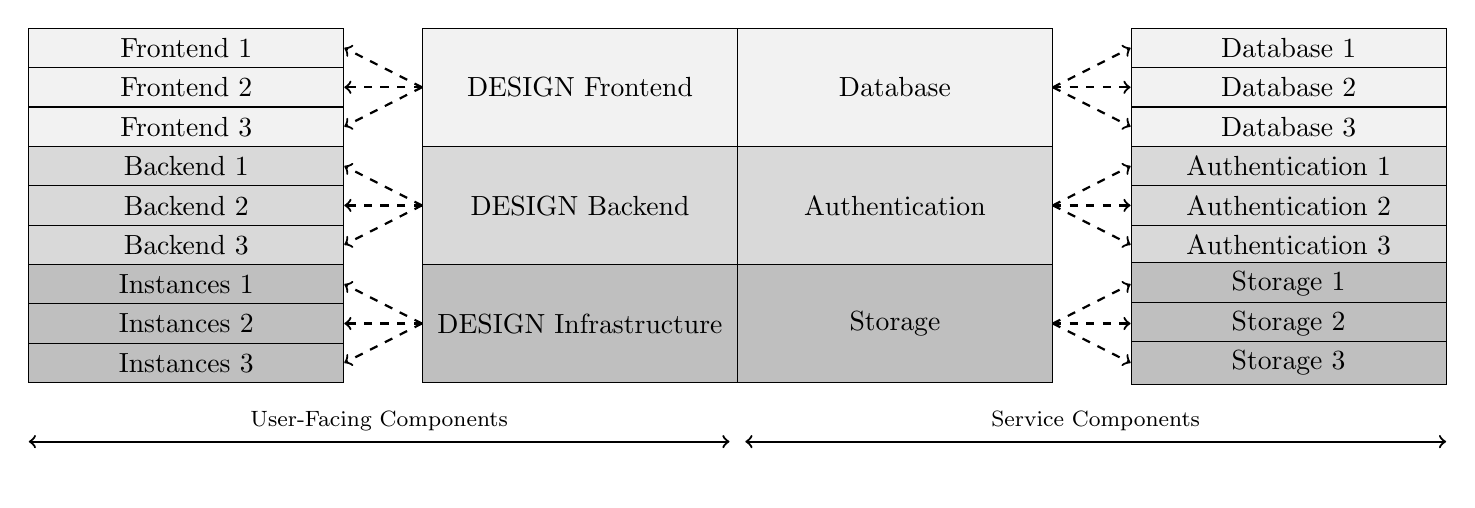
\begin{tikzpicture}[every node/.style={minimum height=1.5cm, align=center}]
			% Node
			\node[draw, minimum width=4cm, fill=gray!10] (front0) at (-4,-3.0) {DESIGN Frontend};
			\node[draw, minimum width=4cm, fill=gray!30] (back0) at (-4,-4.5) {DESIGN Backend};
			\node[draw, minimum width=4cm, fill=gray!50] (inf0) at (-4,-6.0) {DESIGN Infrastructure};
			\node[draw, minimum width=4cm, fill=gray!10] (db0) at (0,-3.0) {Database};
			\node[draw, minimum width=4cm, fill=gray!30] (auth0) at (0,-4.5) {Authentication};
			\node[draw, minimum width=4cm, fill=gray!50] (fs0) at (0,-6.0) {Storage};
			% Frontends
			\node[draw, minimum width=4cm,minimum height=0.5cm, fill=gray!10] (front1) at (-9,-2.5) {Frontend 1};
			\node[draw, minimum width=4cm,minimum height=0.5cm, fill=gray!10] (front2) at (-9,-3.0) {Frontend 2};
			\node[draw, minimum width=4cm,minimum height=0.5cm, fill=gray!10] (front3) at (-9,-3.5) {Frontend 3};
			\draw[->, dashed, thick, black] (front0.west) -- (front1.east);
			\draw[->, dashed, thick, black] (front0.west) -- (front2.east);
			\draw[->, dashed, thick, black] (front0.west) -- (front3.east);
			% Backends
			\node[draw, minimum width=4cm,minimum height=0.5cm, fill=gray!30] (back1) at (-9,-4.0) {Backend 1};
			\node[draw, minimum width=4cm,minimum height=0.5cm, fill=gray!30] (back2) at (-9,-4.5) {Backend 2};
			\node[draw, minimum width=4cm,minimum height=0.5cm, fill=gray!30] (back3) at (-9,-5.0) {Backend 3};
			\draw[->, dashed, thick, black] (back0.west) -- (back1.east);
			\draw[->, dashed, thick, black] (back0.west) -- (back2.east);
			\draw[->, dashed, thick, black] (back0.west) -- (back3.east);
			% Instances
			\node[draw, minimum width=4cm,minimum height=0.5cm, fill=gray!50] (inst1) at (-9,-5.5) {Instances 1};
			\node[draw, minimum width=4cm,minimum height=0.5cm, fill=gray!50] (inst2) at (-9,-6.0) {Instances 2};
			\node[draw, minimum width=4cm,minimum height=0.5cm, fill=gray!50] (inst3) at (-9,-6.5) {Instances 3};
			\draw[->, dashed, thick, black] (inf0.west) -- (inst1.east);
			\draw[->, dashed, thick, black] (inf0.west) -- (inst2.east);
			\draw[->, dashed, thick, black] (inf0.west) -- (inst3.east);
			% DB
			\node[draw, minimum width=4cm,minimum height=0.5cm, fill=gray!10] (db1) at (5,-2.5) {Database 1};
			\node[draw, minimum width=4cm,minimum height=0.5cm, fill=gray!10] (db2) at (5,-3.0) {Database 2};
			\node[draw, minimum width=4cm,minimum height=0.5cm, fill=gray!10] (db3) at (5,-3.5) {Database 3};
			\draw[->, dashed, thick, black] (db0.east) -- (db1.west);
			\draw[->, dashed, thick, black] (db0.east) -- (db2.west);
			\draw[->, dashed, thick, black] (db0.east) -- (db3.west);
			% Auth
			\node[draw, minimum width=4cm,minimum height=0.5cm, fill=gray!30] (auth1) at (5,-4.0) {Authentication 1};
			\node[draw, minimum width=4cm,minimum height=0.5cm, fill=gray!30] (auth2) at (5,-4.5) {Authentication 2};
			\node[draw, minimum width=4cm,minimum height=0.5cm, fill=gray!30] (auth3) at (5,-5.0) {Authentication 3};
			\draw[->, dashed, thick, black] (auth0.east) -- (auth1.west);
			\draw[->, dashed, thick, black] (auth0.east) -- (auth2.west);
			\draw[->, dashed, thick, black] (auth0.east) -- (auth3.west);
			% Fs
			\node[draw, minimum width=4cm,minimum height=0.5cm, fill=gray!50] (fs1) at (5,-5.5) {Storage 1};
			\node[draw, minimum width=4cm,minimum height=0.5cm, fill=gray!50] (fs2) at (5,-6.0) {Storage 2};
			\node[draw, minimum width=4cm,minimum height=0.5cm, fill=gray!50] (fs3) at (5,-6.5) {Storage 3};
			\draw[->, dashed, thick, black] (fs0.east) -- (fs1.west);
			\draw[->, dashed, thick, black] (fs0.east) -- (fs2.west);
			\draw[->, dashed, thick, black] (fs0.east) -- (fs3.west);
			% Arrows Bottom
			\draw[<->, thick, black] (-11,-7.5) -- (-2.1,-7.5) node[midway, above, yshift=-0.5cm, font=\footnotesize] {User-Facing Components};
			\draw[<->, thick, black] (-1.9,-7.5) -- (7,-7.5) node[midway, above, yshift=-0.5cm, font=\footnotesize] {Service Components};
		\end{tikzpicture}
	\end{adjustbox}
	\caption{DESIGN Component Redundancy}\label{service_redundancy}
\end{figure}

\subsubsection{Internal Communication}
After discussing the principles of scalability and redundancy,
we finally describe how communication flows are managed within our system.
Our solution is rooted in a message-oriented architecture
designed to fulfill DaaS properties for scalability and redundancy,
as previously outlined.

This implies that any action triggered, whether in the frontend on the client side,
in the backend on the host side or within hosted instances,
must ensure that all necessary information is readily available at the time of processing.

We achieve this by storing runtime information in distributed block storage,
relevant configuration files in distributed file storage,
object metadata in a common database,
and by utilizing a decentralized authentication component.

This ensures that any change triggered by a node within the DaaS domain
is immediately available to any other node relying in some way
on that particular information change.
Additionally, any extra information needed by a component must be fully contained
within the related request.
As shown in figure~\ref{message_routing}, this enables arbitrarily distributed configurations as long as request
and response messages reach their desired target eventually.

If that is the case, each distributed host system might only contain its essential components,
including the backend service with all hosted instances
as well as the described proxy component for direct user interaction.
Any other component may reside somewhere in the DaaS network.

\begin{figure}
	\centering
	\begin{adjustbox}{width=\textwidth}
		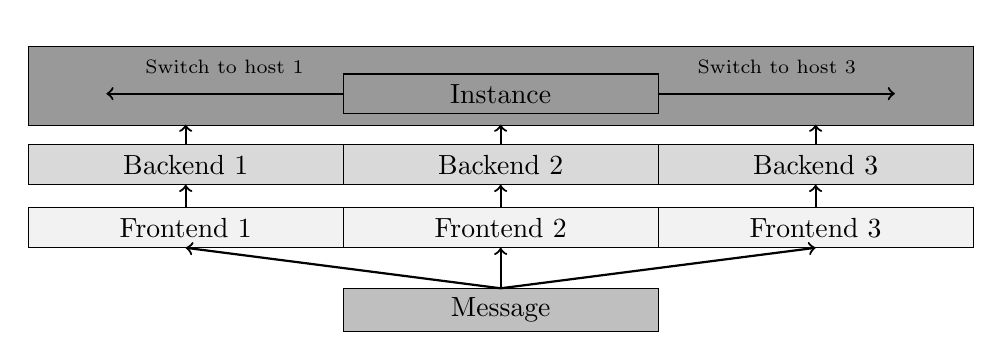
\begin{tikzpicture}[every node/.style={minimum width=4cm, minimum height=1cm, align=center}]
			% Frontends
			\node[draw,minimum height=0.5cm, fill=gray!10] (front1) at (-4,0.3) {Frontend 1};
			\node[draw,minimum height=0.5cm, fill=gray!10] (front2) at (0,0.3) {Frontend 2};
			\node[draw,minimum height=0.5cm, fill=gray!10] (front3) at (+4,0.3) {Frontend 3};
			% Backends
			\node[draw,minimum height=0.5cm, fill=gray!30] (back1) at (-4,1.1) {Backend 1};
			\node[draw,minimum height=0.5cm, fill=gray!30] (back2) at (+0,1.1) {Backend 2};
			\node[draw,minimum height=0.5cm, fill=gray!30] (back3) at (+4,1.1) {Backend 3};
			% Instances
			\node[draw,minimum width=12cm, minimum height=1cm, fill=gray!80] (instdomain) at (+0,2.1) {};
			\node[draw,minimum height=0.5cm, fill=gray!80] (inst) at (+0,2) {Instance};
			% Message
			\node[draw,minimum height=0.5cm, fill=gray!50] (message) at (0,-0.75) {Message};
			% Arrows instance
			\draw[->, thick, black] (inst.west) -- ++(-3,0) node[midway, above=-5pt, font=\scriptsize] {Switch to host 1};
			\draw[->, thick, black] (inst.east) -- ++(3,0) node[midway, above=-5pt, font=\scriptsize] {Switch to host 3};
			% Arrows backend
			\draw[->, thick, black] (back1.north) -- ++(0,0.25);
			\draw[->, thick, black] (back2.north) -- ++(0,0.25);
			\draw[->, thick, black] (back3.north) -- ++(0,0.25);
			% Arrows frontend
			\draw[->, thick, black] (front1.north) -- (back1.south);
			% \draw[->, thick, black] (front1.north) -- (back2.south);
			% \draw[->, thick, black] (front1.north) -- (back3.south);
			% \draw[->, thick, black] (front2.north) -- (back1.south);
			\draw[->, thick, black] (front2.north) -- (back2.south);
			% \draw[->, thick, black] (front2.north) -- (back3.south);
			% \draw[->, thick, black] (front3.north) -- (back1.south);
			% \draw[->, thick, black] (front3.north) -- (back2.south);
			\draw[->, thick, black] (front3.north) -- (back3.south);
			% Arrows Message
			\draw[->, thick, black] (message.north) -- (front1.south);
			\draw[->, thick, black] (message.north) -- (front2.south);
			\draw[->, thick, black] (message.north) -- (front3.south);
		\end{tikzpicture}
	\end{adjustbox}
	\caption{Message Oriented Routing.}\label{message_routing}
\end{figure}

\subsection{Usability}
An essential feature of a DaaS platform is its strong user-friendliness,
which eliminates the complexity of the different operating systems
used inside virtual machines and containers,
makes the underlying hardware transparent,
and simplifies the necessary interactions as much as possible.

Since users already have an operating system on their clients,
and the motivation for using a DaaS is the simple use of various applications,
it makes no sense for most users to have additional desktops available in the browser.
The focus should be on the applications.
For this reason, when developing a new DaaS solution,
the main goal should be to reduce the graphical output
to the limits of the respective application.
The concept uses a separate browser tab for each application
whose content exclusively represents the application.

Developing the automatic adaptation of the output
to the limits of the respective application window is challenging.
Only a few RDP and VNC server implementations offer to export the graphical output
of only individual windows or processes.
For Windows operating systems, the proprietary built-in RDP server
and the free software TightVNC offer the export of full desktops and single windows.

For Linux operating system deployments,
the free software projects xrdp and x11vnc enable all desired features
and single-app functionality can be easily obtained
by using a custom window manager such,
as for example, qtile\footnote{\url{https://qtile.org}}.

Table~\ref{tab:DaaS_Services_Overview} includes an overview
of the mentioned service implementations for RDP and VNC protocols
and their relevant characteristics.
Further implementations like TigerVNC and protocols like NX NoMachine exist
but do not seem useful for designing and implementing a novel DaaS because
they do not meet all feature requirements~\cite{OJCC_2023v8i1n01_Baun}.

\begin{table}
	\centering
	\caption{Services used by our DaaS for Remote Access to individual Applications}
	\begin{tabular}{|l|c|c|c|c|}
		\hline
		\textbf{Service}        & \textbf{Protocol} & \textbf{Single Window} & \textbf{Operating} & \textbf{Software} \\
		\textbf{implementation} &                   & \textbf{Mode}          & \textbf{System}    & \textbf{License}  \\
		\hline
		TightVNC                & VNC               & supported              & Windows            & GPL2              \\
		\hline
		Windows RDP server      & RDP               & supported              & Windows            & proprietary       \\
		\hline
		x11vnc                  & VNC               & not supported          & Linux              & GPL2              \\
		\hline
		Xrdp                    & RDP               & supported              & Linux              & Apache 2.0        \\
		\hline
	\end{tabular}
	\label{tab:DaaS_Services_Overview}
\end{table}

The automatic adaptation of viewer size and screen resolution,
considering underlying protocols and systems,
faced various limitations, briefly described below.

One challenge was imposed by Guacamole's current lack of support
for dynamic desktop resizing with VNC,
leading to misaligned layouts and a poor user experience.
To address this until such features are available in
Guacamole\footnote{\url{https://issues.apache.org/jira/browse/GUACAMOLE-1196}},
we implemented a separate mechanism using a WebSocket proxy
and direct interaction with each instance.

Additionally, protocol-specific behaviors may vary
when hosted on different platforms or infrastructures.
For instance, we observed connection terminations when resizing Linux-based containers,
contrasting with the behavior observed in equivalent Linux-based virtual machines.
To overcome such limitations, we created a separate layer around the Guacamole client,
adapting to each infrastructure, platform, or protocol-specific configuration.

Another challenge was managing RDP sessions, which are typically tied to actual users,
unlike VNC sessions, which are typically authenticated against
a server-maintained user registry.
Utilizing the WebSocket proxy, the backend could pass credentials
to the server without revealing them to the user.

Essentially, Guacamole, with its protocol implementations and additional features like audio and printing,
provided the fundamental base for our core capabilities.

Finally, certain instances might not be fully accessible during runtime
due to hardware malfunctions and inappropriate system configurations during system updates.
Therefore, as a failover mechanism, additional logic had to be added
to provide reasonable debug views and recovery mechanisms,
e.g., recreate instances from a specific snapshot or configuration state.

A crucial lesson learned was, therefore, to realize that
while individual problems can mostly be solved
using established paradigms, services, or libraries with only slight modifications,
the real challenge for a full-fledged DaaS system lies in its abilities
to combine such isolated solutions appropriately
and for each specific infrastructure and platform configuration.

\section{Conclusion and Outlook}\label{sec:Conclusions}

In this paper, we describe an architecture for a novel
and feature-rich DaaS that is, by principle,
superior to comparable products and approaches
because it supports running unmodified Linux and Windows applications.
Furthermore, we identified characteristic issues
-- concerning compatibility, performance, stability, and usability --
during the development and implementation of our DaaS
and present solutions to overcome these challenges.

For future work,
we plan to replace our temporary solution for internal communication
with a more efficient approach as our preliminary performance tests revealed
a potential bottleneck in that particular area.
We also plan to apply certain optimization strategies
concerning backend and instance communication.
We further plan to enhance our yet limited performance testing
and will provide a full-fledged performance analysis
of realistic deployment scenarios and utilization patterns
which include an evaluation of different user behaviors
within various popular applications.

\section*{Acknowledgements}

The Federal Ministry for Economic Affairs and Climate Action funded this work
('\textsl{Bundesministerium f\"ur Wirtschaft und Klimaschutz}')
in the framework of the central innovation programme
for small and medium-sized enterprises
('\textsl{Zentrales Innovationsprogramm Mittelstand}').

We thank our project partners from Nuromedia GmbH for their support.
We especially thank Björn Goetschke, Mike Ludemann, Dario Savella, Holger Sprengel, and Rahul Tomar.

% ---- Bibliography ----
\bibliographystyle{splncs04}
\bibliography{biblio}

\end{document}
